\documentclass[12pt]{article}

\setlength{\parskip}{1em}

\usepackage[T1]{fontenc}
\usepackage[a4paper, margin=0.7in]{geometry}
\usepackage{amsfonts}
\usepackage{mathabx}
\usepackage{listings}
\usepackage{xcolor}
\usepackage{subcaption}
\usepackage{multirow}
\usepackage{makecell}
\usepackage{graphicx}

\usepackage{hyperref}
\hypersetup{
  colorlinks=true,
  linkcolor=blue,
  urlcolor=blue,
  pdftitle={AP4B Project: Power Sim}
}

\definecolor{bgColor}{rgb}{0.95,0.95,0.92}
\lstdefinestyle{Java}{
    backgroundcolor=\color{bgColor},
    commentstyle=\color{gray},
    keywordstyle=\color{magenta},
    numberstyle=\tiny\color{gray},
    stringstyle=\color{purple},
    basicstyle=\footnotesize,
    breakatwhitespace=false,
    breaklines=true,
    captionpos=b,
    keepspaces=true,
    numbers=left,
    numbersep=5pt,
    showspaces=false,
    showstringspaces=false,
    showtabs=false,
    tabsize=2,
    language=JAVA
}

\graphicspath{{report/}}

\title{Projet d'AP4B: Power Sim}
\author{
    Osée Tchappi \\
    Adrien Burgun \\
    Tarabai Gambara \\
    Jiang YiWen
}
\date{Automne 2021}

\begin{document}
\maketitle

\begin{abstract}
    Pour ce projet d'AP4B, nous avons décidé de choisir le sujet "Power Sim".
\end{abstract}

\newpage
\tableofcontents
\newpage

\section{Cas d'utilisations}

\section{Diagramme de Classe}

Nous avons construit un diagramme de classe, implémentant les besoins émis dans le diagramme de cas d'utilisation et servant de base aux diagrammes de séquences venant par la suite.
Celui-ci a été découpé en plusieurs sous-diagrammes pour la lisibilité; le diagramme complet peut être trouvé sur GitHub: \url{https://github.com/adri326/ap4b-project/}

Dans cette conception du projet, la classe \texttt{GameState} est la classe principale de la méchanique du jeu: celle-ci stoque l'entièreté des informations d'une partie.
Les différents composants de cette classe correspondent aux différents besoins du projet:

\begin{itemize}
\item La classe \texttt{Tile} (Figure~\ref{fig:tile}, contenue dans la classe \texttt{Map}) est commune à tous les bâtiments posés sur l'espace de jeu: celle-ci est étendue pour implémenter la logique et les spécificités des différents bâtiments (Figure~\ref{fig:factory}).
\item La classe \texttt{Bank} gère la partie "banque": rémunérer le joueur au début, faire un prêt, etc.
\item La classe \texttt{Simulation} gère le coeur de la simulation du jeu: l'immigration, la génération de resources et la pollution.
\item La classe \texttt{Weather} contient une petite simulation de météo et du cycle jour/nuit.
\item La classe \texttt{TechTree} (Figure~\ref{fig:techtree}) contient les technologies que le joueur débloque au fil de la partie: celles-cis sont caractérisées par des pré-requis (\texttt{Requirement}) et des récompenses (\texttt{Reward}).
\end{itemize}

Les classes spécifiques à la partie graphisme sont incluses dans ce rapport mais seront amenées à être modifiées et étendues lors de la phase d'implémentation du projet. Celles-cis se trouve dans la Figure~\ref{fig:application}

\begin{figure}[ht]
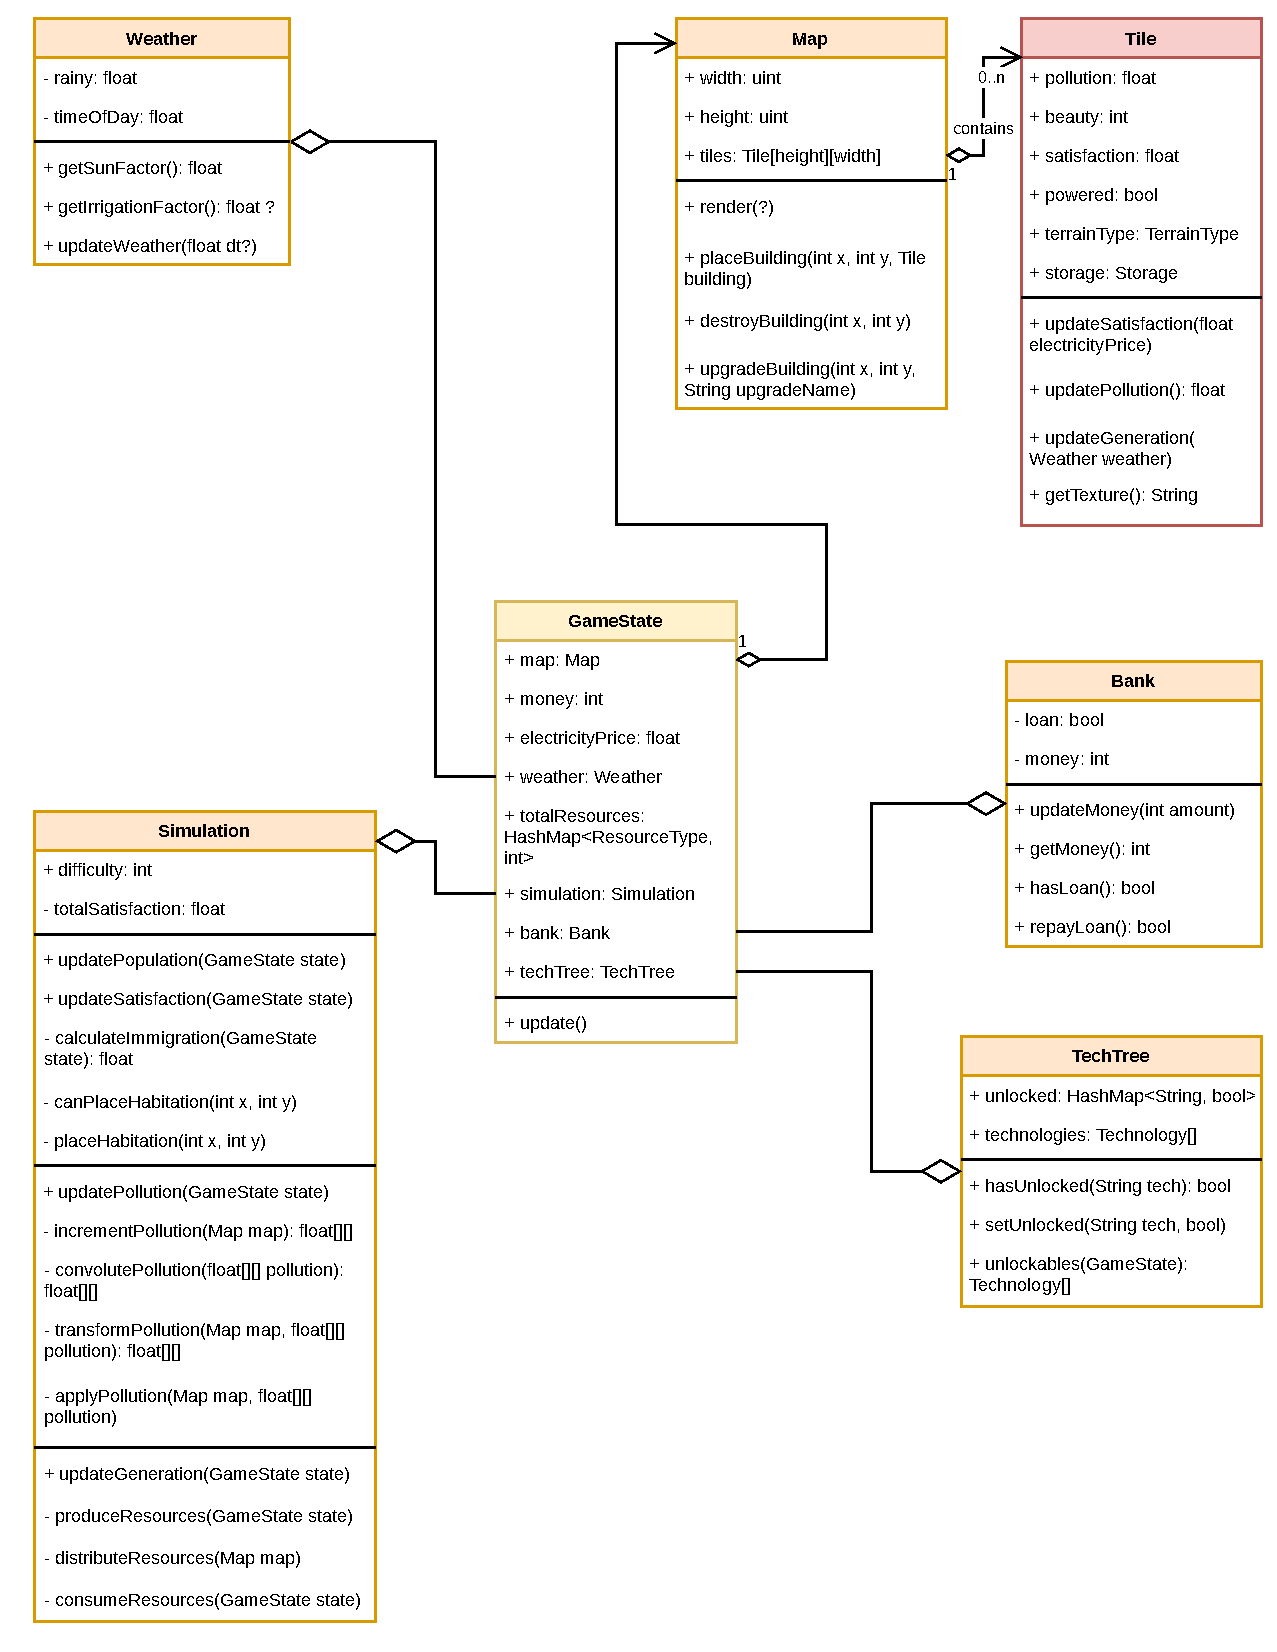
\includegraphics[width=\textwidth]{uml-classes-Page-2}
\caption{La classe principale \texttt{GameState} et les classes qu'elle contient.\label{fig:gamestate}}
\end{figure}

\begin{figure}[ht]
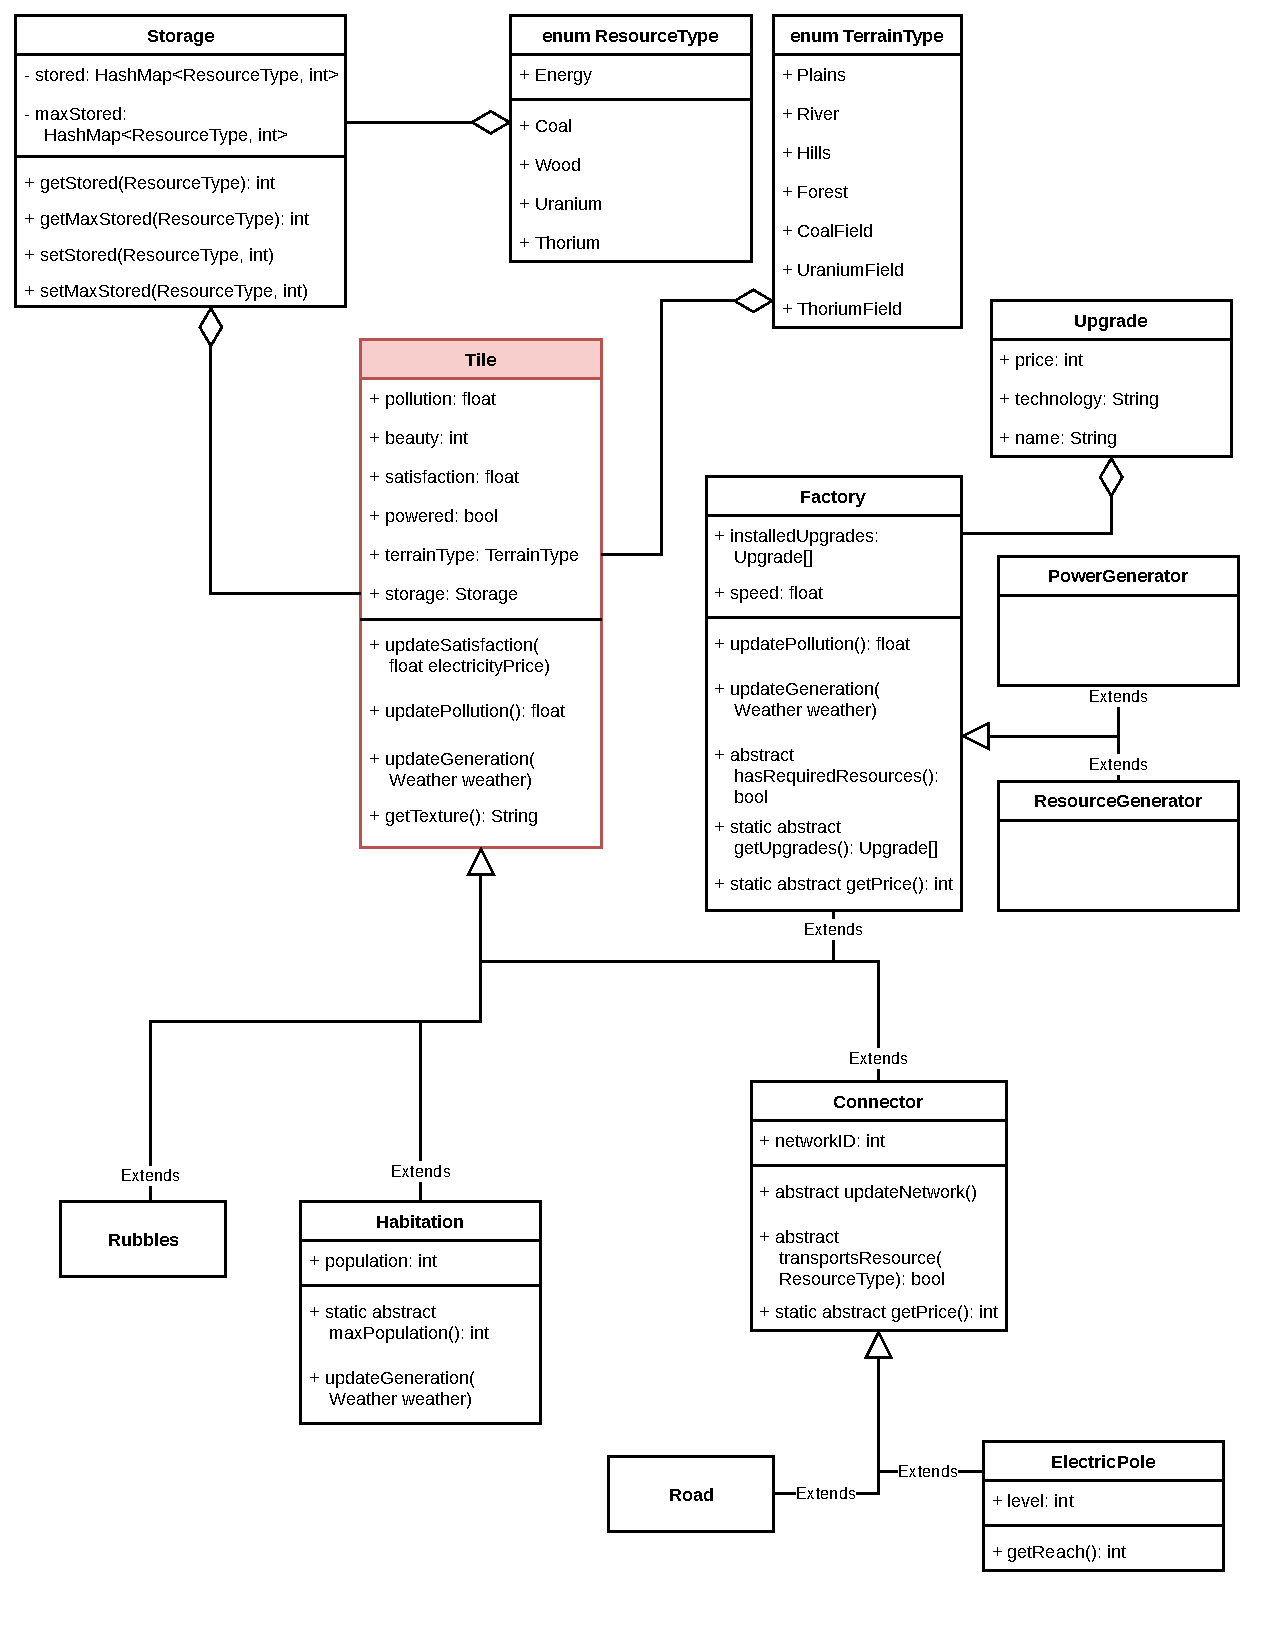
\includegraphics[width=\textwidth]{uml-classes-Page-3}
\caption{La classe \texttt{Tile} et ses principaux descendants.\label{fig:tile}}
\end{figure}

\begin{figure}[ht]
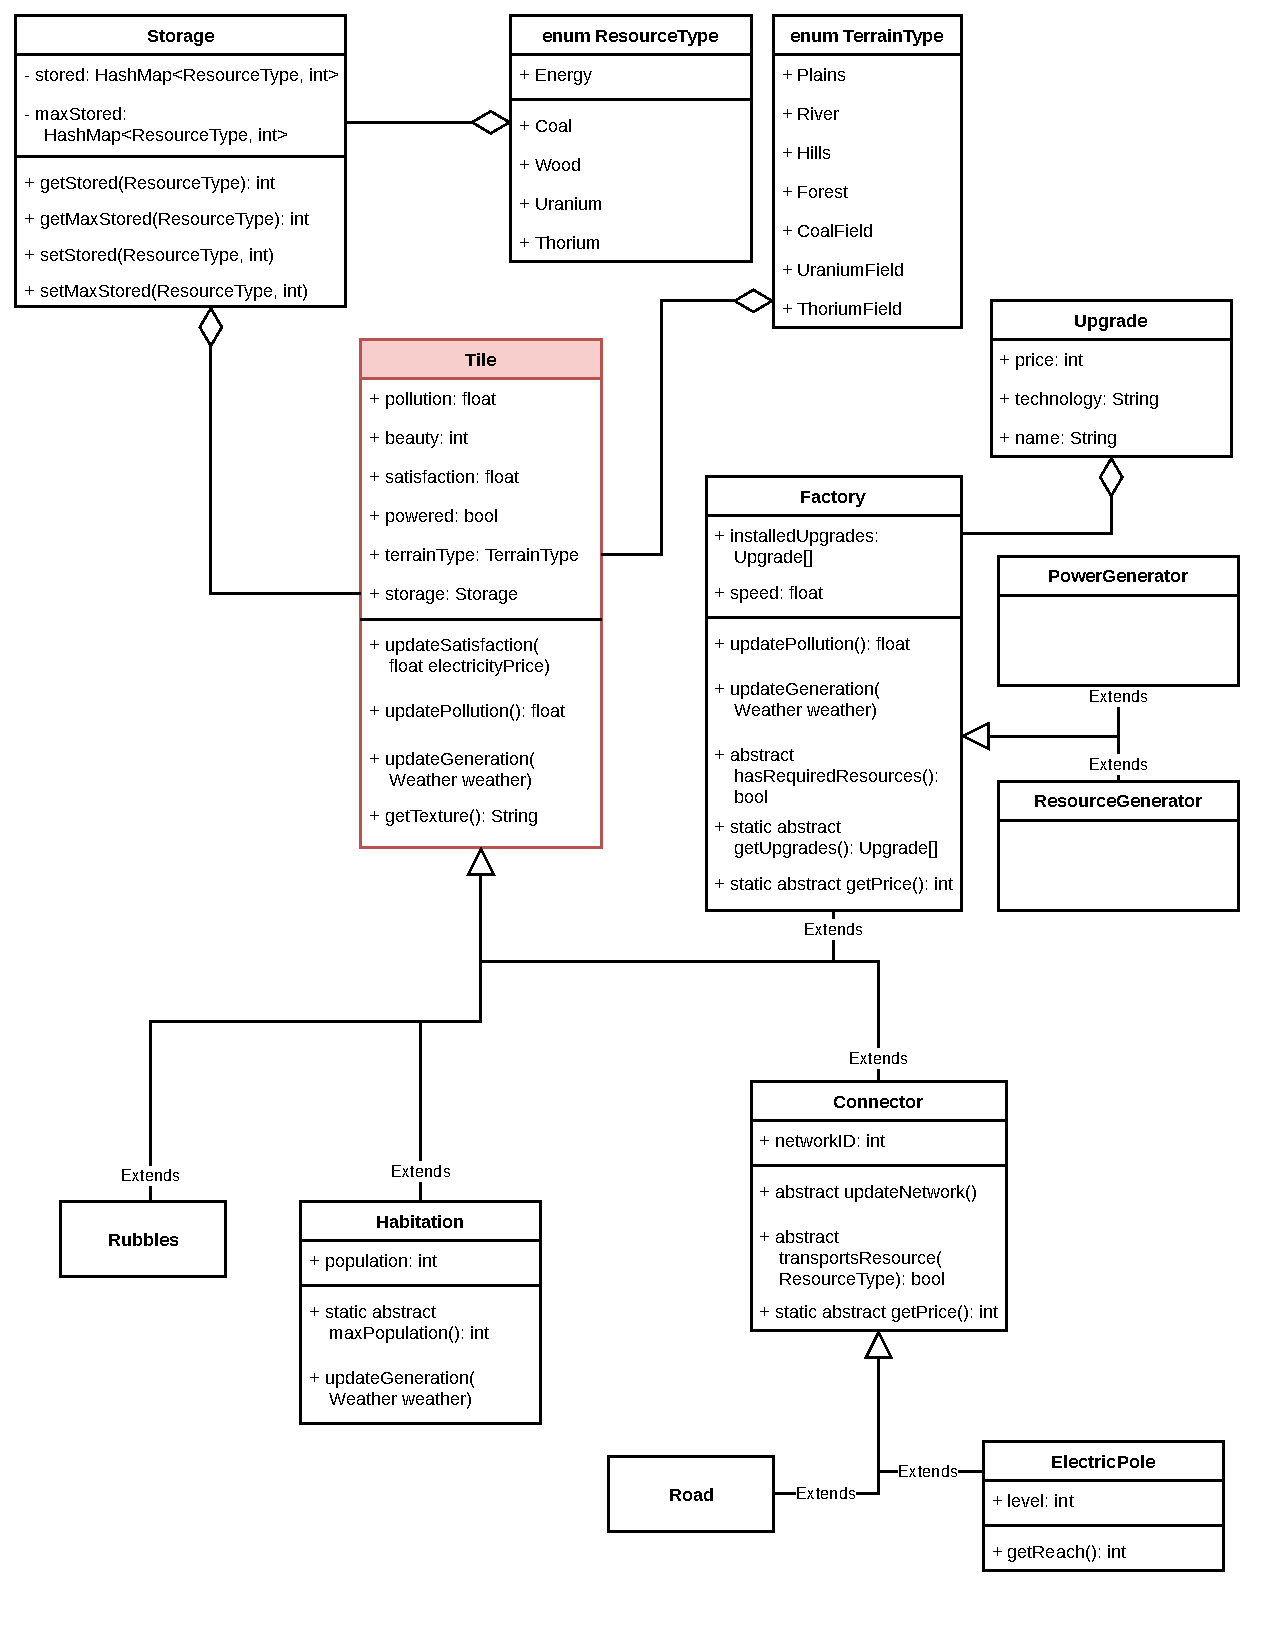
\includegraphics[width=\textwidth]{uml-classes-Page-3}
\caption{Détail de Figure~\ref{fig:tile}: les classes descendant de \texttt{Factory} et de \texttt{Habitation}.\label{fig:factory}}
\end{figure}

\begin{figure}[ht]
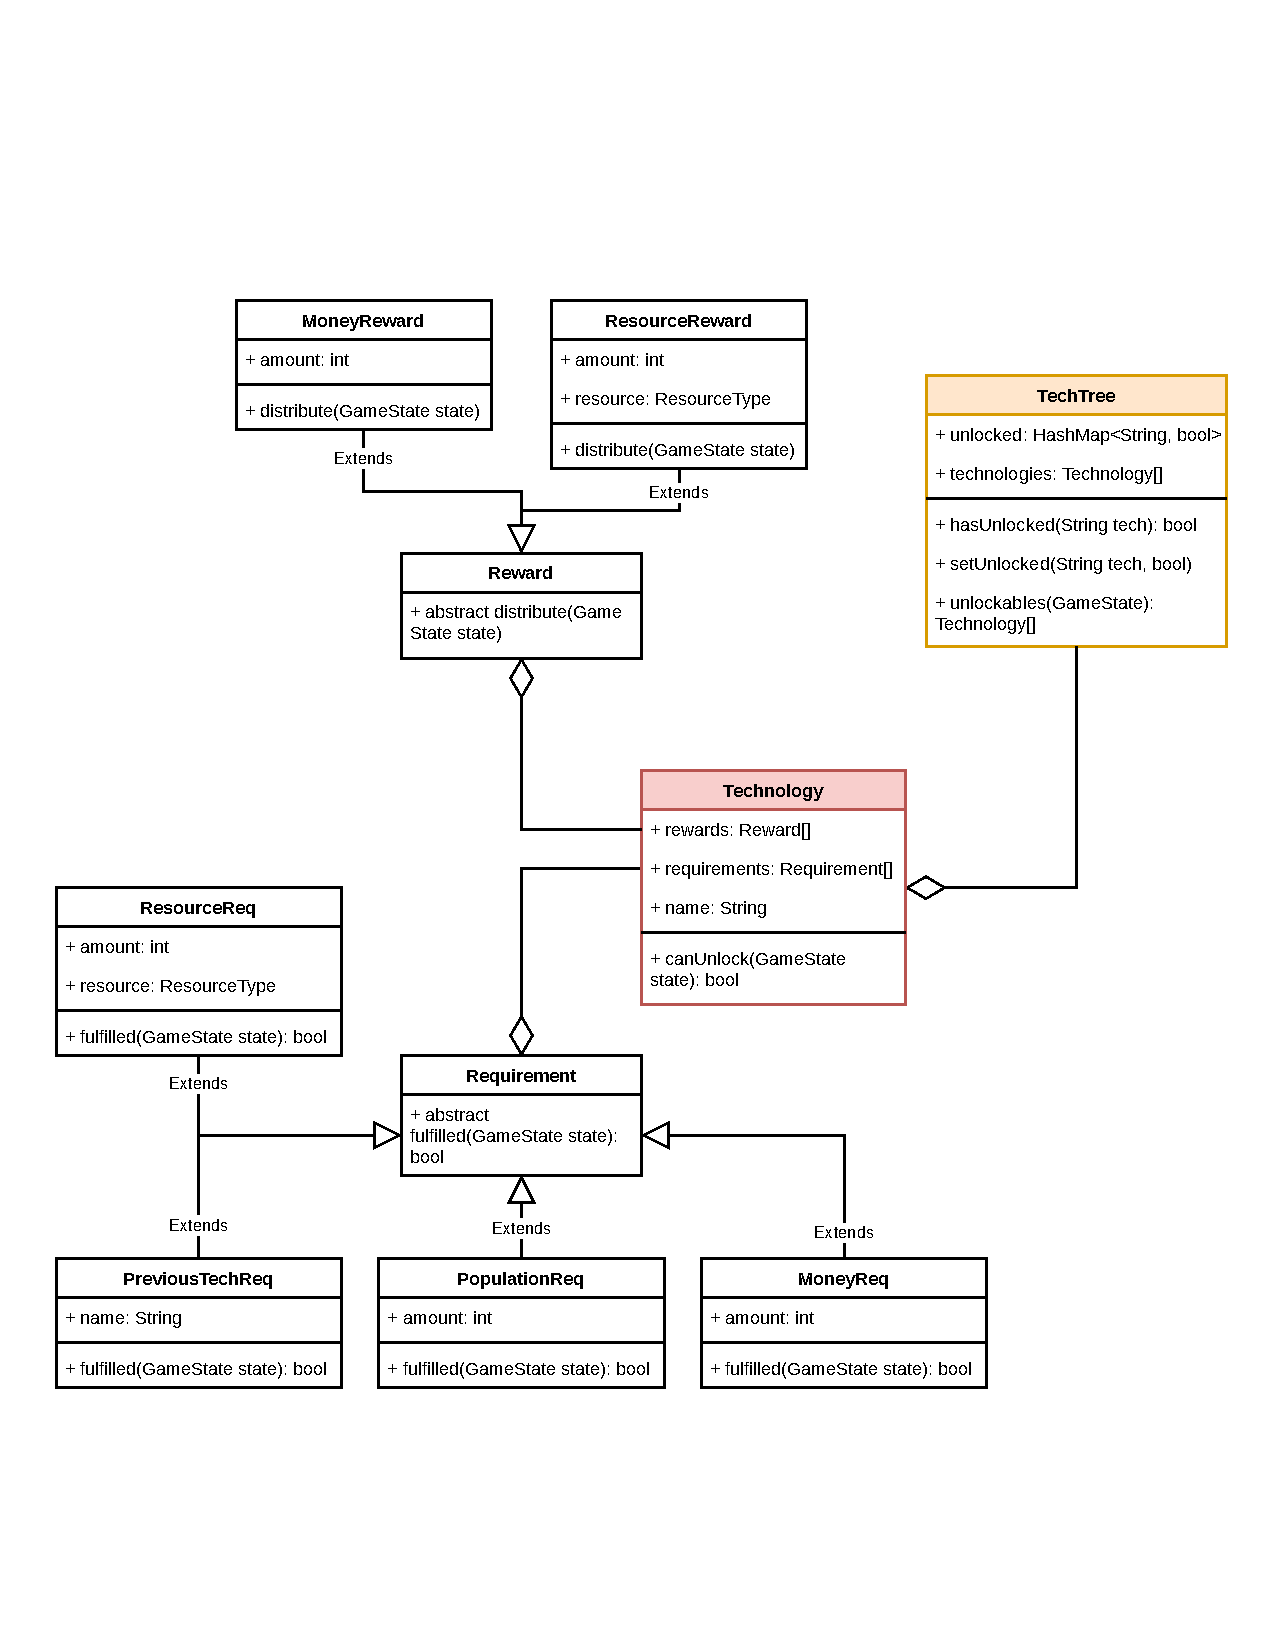
\includegraphics[width=\textwidth]{uml-classes-Page-5}
\caption{La classe \texttt{TechTree} et ses principaux descendants.\label{fig:techtree}}
\end{figure}

\begin{figure}[ht]
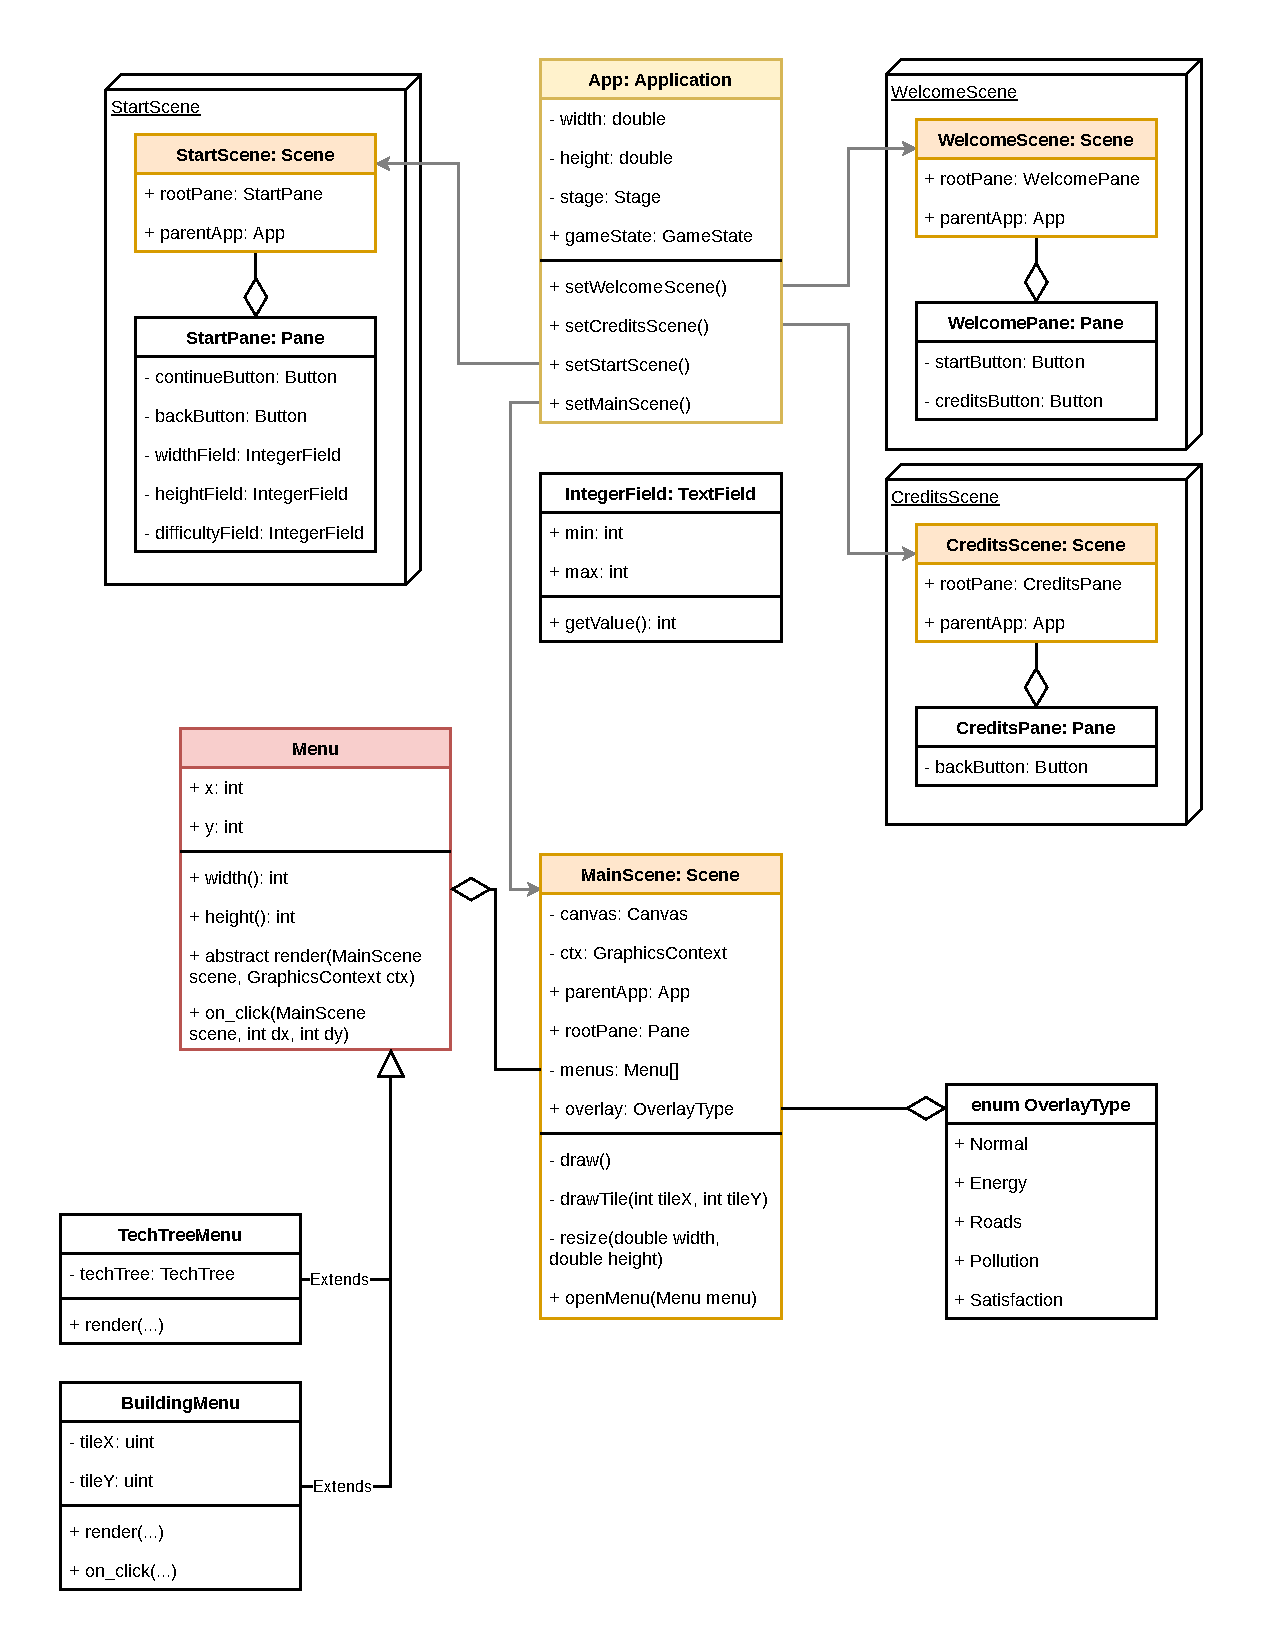
\includegraphics[width=\textwidth]{uml-classes-Page-6}
\caption{La classe \texttt{App} et les différentes classes pour l'affichage du jeu.\label{fig:application}}
\end{figure}

\end{document}
